%%%%%%%%%%%%%%%%%%%%%%%%%%%%%%%%%%%%%%%%%%%%%%%%%%%%%%%%%%%%%%%%%%%%%%%%%%%%%%%%
% Chapter 4: Desarrollo
%%%%%%%%%%%%%%%%%%%%%%%%%%%%%%%%%%%%%%%%%%%%%%%%%%%%%%%%%%%%%%%%%%%%%%%%%%%%%%%%

%+++++++++++++++++++++++++++++++++++++++++++++++++++++++++++++++++++++++++++++++
% \section{Desarrollo en Perenquén
% \label{4:sec:3}

Como se ha señalado en la sección anterior, la odometría visual no es suficiente
para un sistema de navegación robusto. La silla Perenquén ofrece odometría
mecánica y oodmetría láser, por lo que entre las tres ofreceran mejores
resultados.

%+++++++++++++++++++++++++++++++++++++++++++++++++++++++++++++++++++++++++++++++
\subsection{Introducción}

\begin{wrapfigure}{l}{0.25\textwidth}
  \vspace{-20pt}
  \begin{center}
    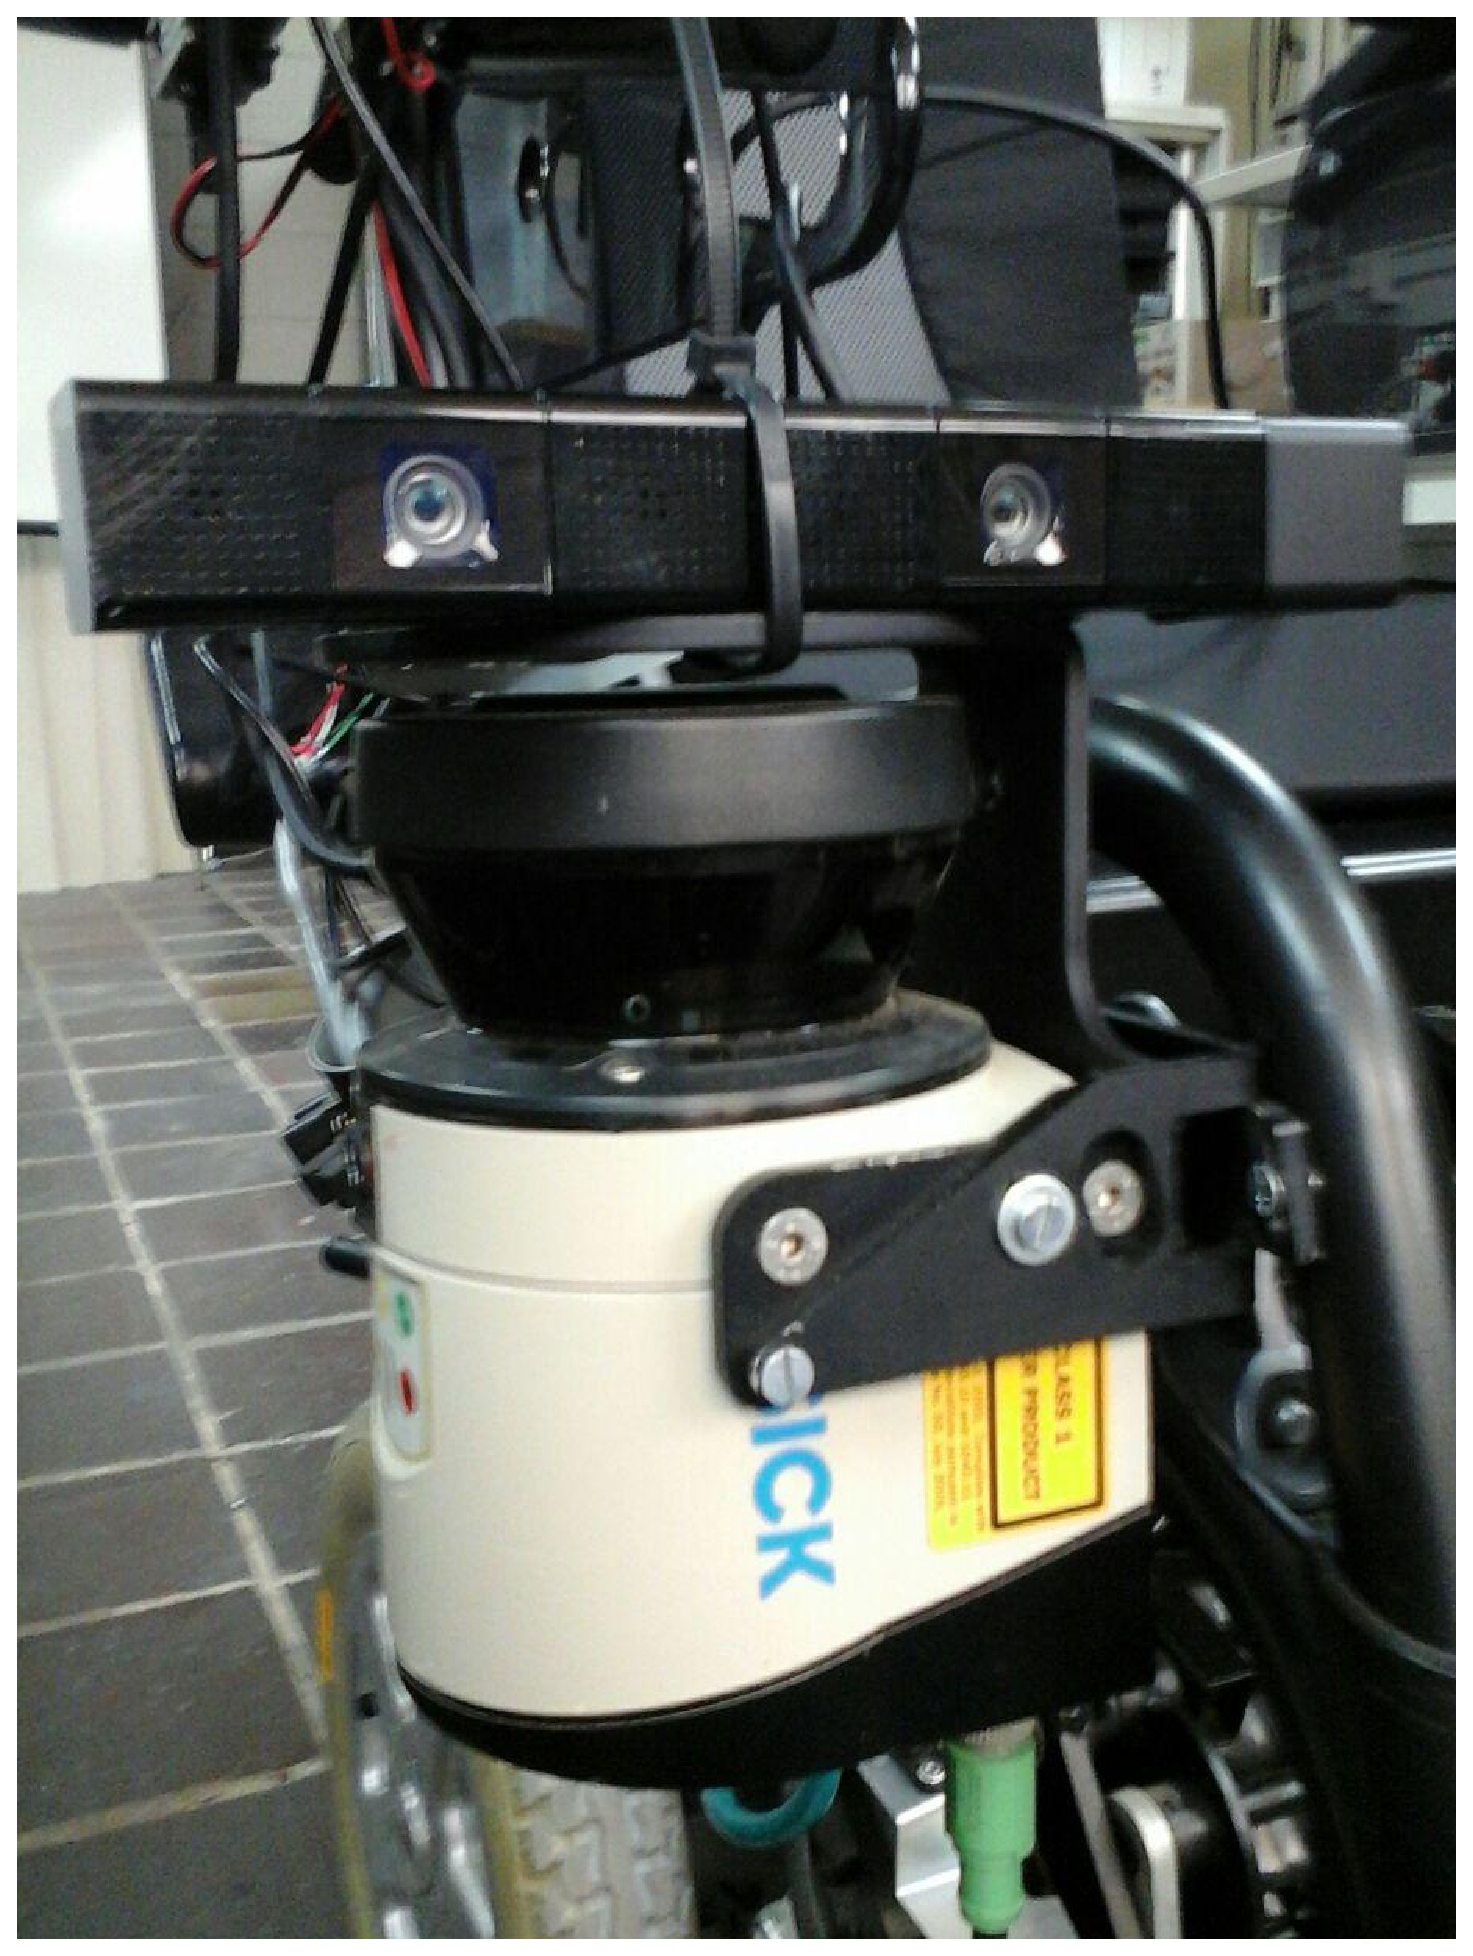
\includegraphics[width=0.24\textwidth]{images/cap4/Perenquen-camara.eps}
  \end{center}
  \vspace{-20pt}
  \caption{PlayStation Camera en la silla Perenquén}
  \vspace{-10pt}
  \label{fig:Perenquen-Camara}
\end{wrapfigure}

Al igual que sucedió anteriormente, el objetivo sigue está en reconstruir un
mapa en tres dimensiones a través de las imágenes capturadas por PlayStation
Camera, aunque en esta ocasión, no solamente la cámara estará conectada con el
ordenador, también la silla Perenquén estará conectada a él. La silla destaca
por contar con un sistema de odometría mecánica y tres sistemas láser, uno a
cada lado y otro en la parte trasera.

En esta ocasión no solo se va trabajar con bolsas de datos ya grabadas, también
se trabajará en recoger y analizar las imágenes en tiempo real. De esta forma,
es necesario modificar las instrucciones descritas en el archivo de
configuración utilizado hasta el momento ~\ref{appendix:carrito}, añadiendo principalmente la adquisición e integración del resto de sistemas de odometría.

%+++++++++++++++++++++++++++++++++++++++++++++++++++++++++++++++++++++++++++++++
\subsection{Integración de los sistemas de odometría}

Ahora la idea general para la reconstrucción del mapa tridimensional pasa por:

\begin{itemize}
  \item Ajustar cámara y obtener imágenes en estéreo
  \item Obtener una odometría a partir de la visual, mecánica y láser
  \item Construir el mapa
\end{itemize}

\begin{minipage}{\linewidth}
    \centering
    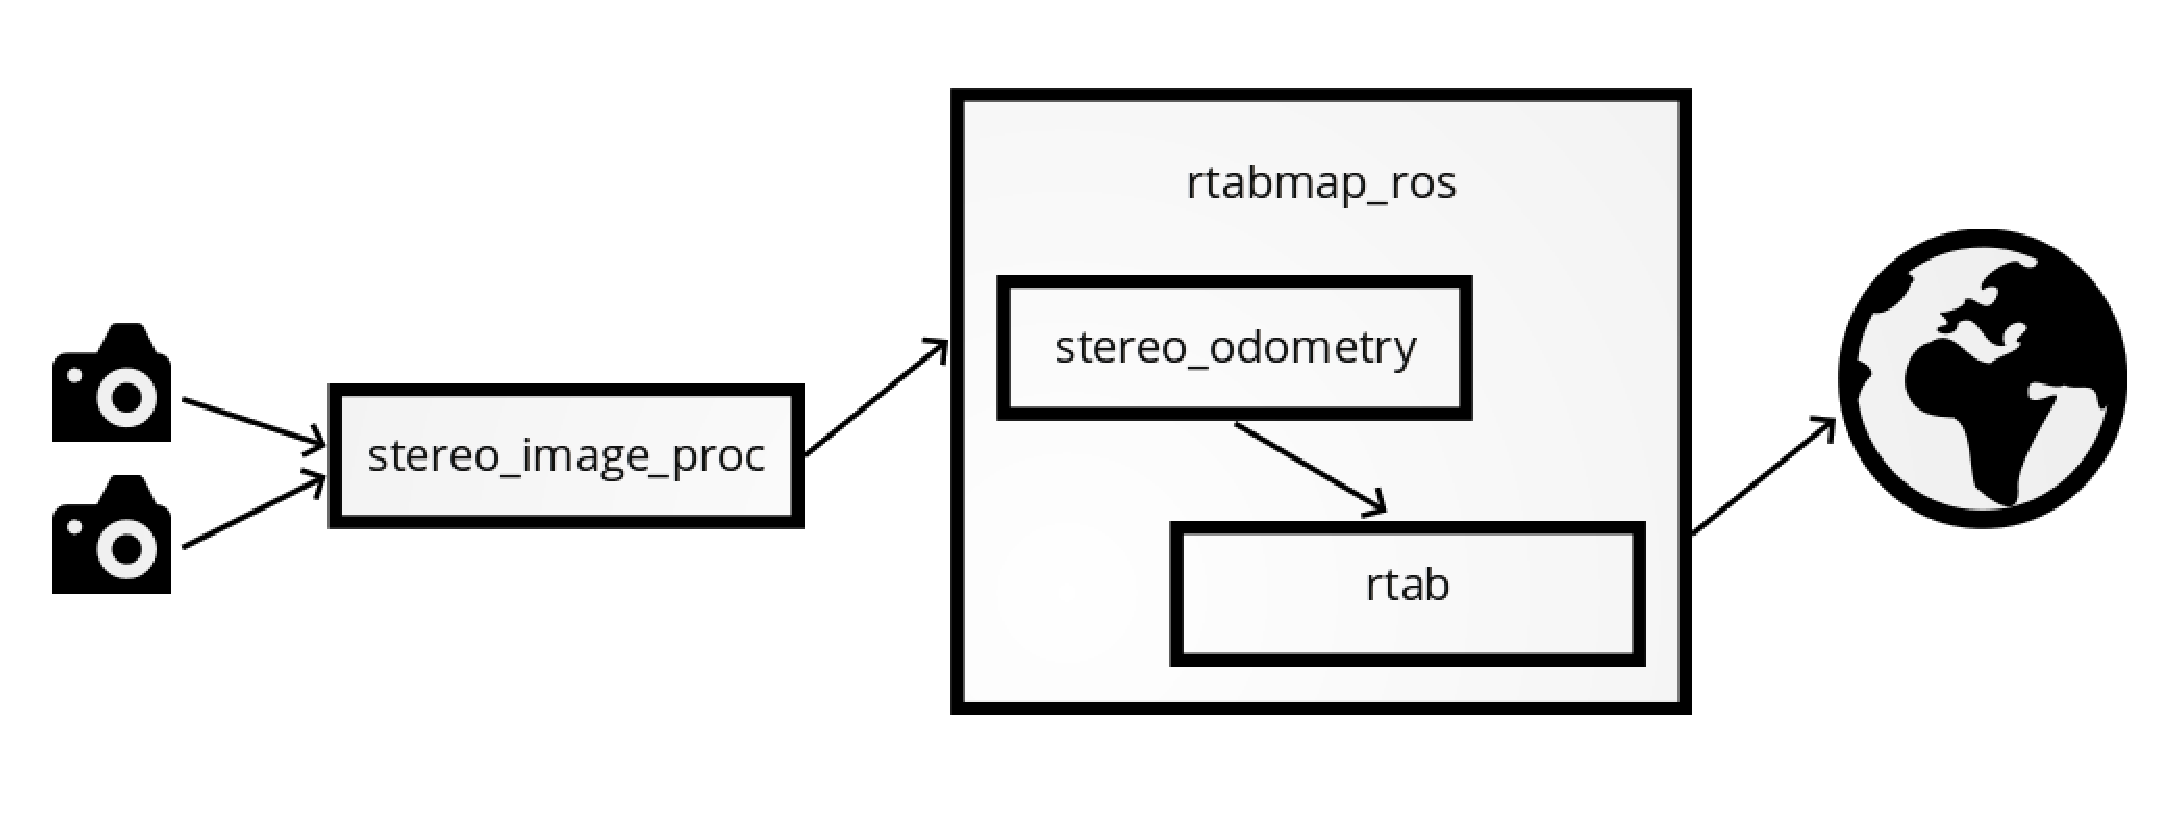
\includegraphics[width=0.8\textwidth]{images/cap4/Carro-esquema.eps}
    \captionof{figure}{Esquema de ROS para construir un mapa 3D integrando las
    odometrías.}
    \label{fig:Carro-esquema}
\end{minipage}

%--------------------------------------
\paragraph{Ajustar cámara} \hspace{0pt}

% http://www.slideshare.net/ssuser4d25e1/20160126-jetson-ps4eye01
% http://wiki.ros.org/gscam
% http://wiki.ros.org/image_proc#image_proc.2BAC8-cturtle.image_proc
Para poder capturar imágenes directamente desde PlayStation Camera es necesario
utilizar el paquete de ROS 'ps4eye' que se instaló previamente. Este paquete
dispone de dos utilidades muy importantes, por un lado un script para la
calibración de las cámaras y por otro lado la descomposición de los datos que
obtienen ambas cámaras, en dos imágenes diferentes.

Aunque se podría pensar, que cada cámara debería capturar una imagen a su
resolución nativa, por ejemplo dos imágenes con una resolución de 640x400
píxeles cada una, la realidad es muy diferente. Si se intenta utilizar
PlayStation Camera como una webcam tradicional, el resultado en este caso sería
una sola imagen con una resolución de 1748x408 píxeles.

Es necesario utilizar el paquete de ROS 'gscam'. Se trata de un driver que
permite utilizar el framework multimedia GStreamer para conectar cualquier
dispositivo de vídeo, como en este caso PlayStation Camera. A este paquete solo
es necesario especificarle las características de la cámara: de que dispositivo
se trata, el formato de las imágenes, la resolución de captura y la tasa de
fotogramas por segundo. De esta forma podemos acceder a la imagen raw que arroja
PlayStation Camera.

Posteriormente, se necesita convertir en dos imágenes separadas. Para ello se
utiliza el paquete 'image\_proc'. Este paquete es muy similar al de
'stereo\_image\_proc', sin embargo este trabaja solamente con una imagen.
Contiene un nodo con el mismo nombre cuyo objetivo principal es el de rectificar
la imagen. Sin embargo, el principal interés radica en la disponibilidad de una
utilidad denominada 'image\_proc/crop\_decimate que recibe la imagen de la
cámara y permite obtener una imagen nueva a partir de recortar y ajustar la
imagen original según las necesidades. En este caso, se desea obtener una nueva
imagen izquierda y derecha, cuya resolución será de 640x480.

Si se lanza la herramienta 'image\_view' es posible observar las dos nuevas
imágenes correspondiente a lo que ve la cámara izquierda y la derecha a partir
de la imagen original. Esto se puede observar en el launch correspondiente
descrito aquí.% ~\ref{appendix:perenquen-stereo}.

%--------------------------------------
\paragraph{Calibración} \hspace{0pt}
% http://wiki.ros.org/camera_calibration

En el caso anterior, para poder obtener las dos nuevas imágenes es necesario que
las cámaras estén ya calibradas. La calibración es el proceso en el que se
comparan los valores reales obtenidos por las cámaras respecto a las de un
patrón de referencia. La formas habitual para realizar esto, es utilizando el
método de calibrazión de Zhang, mediante un plano 2D previamente establecido. 

\begin{wrapfigure}{r}{0.5\textwidth}
  \vspace{-20pt}
  \begin{center}
    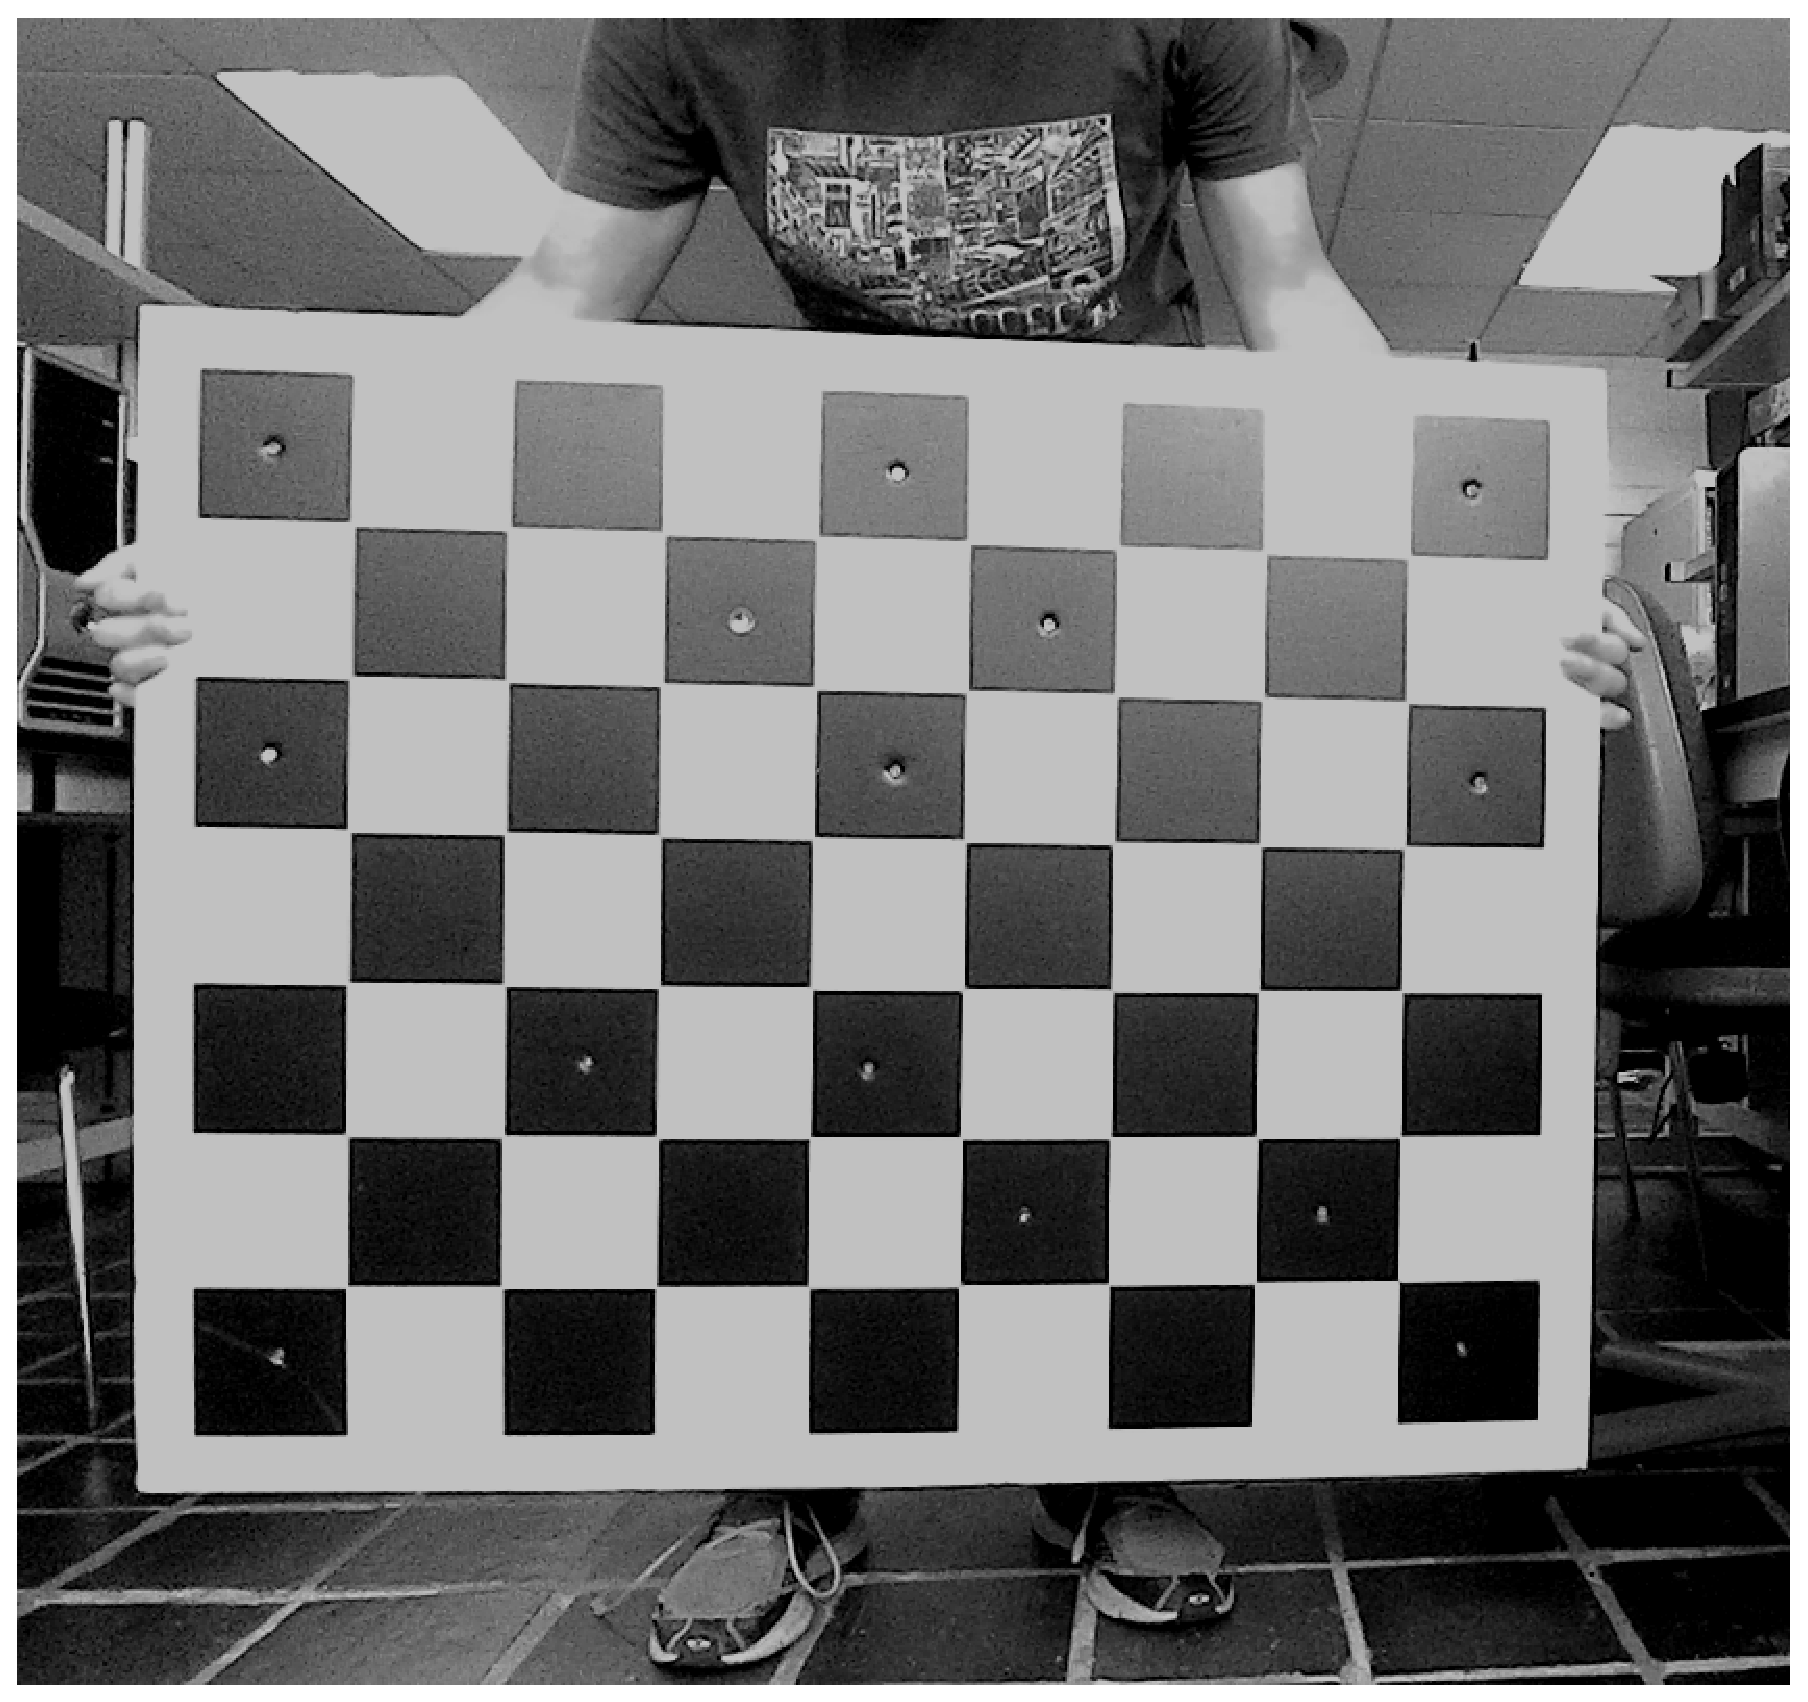
\includegraphics[width=0.48\textwidth]{images/cap4/Calibracion.eps}
  \end{center}
  \vspace{-20pt}
  \caption{Calibración de las cámaras.}
  \vspace{-10pt}
  \label{fig:Calibracion}
\end{wrapfigure}

En ROS existe el paquete de 'camera\_caliration', el cuál permite calibrar de
una manera muy sencilla cualquier cámara monocoluar o estéreo mediante el uso de
un tablero de de damas o ajedrez como el de la figura ~\ref{fig:Calibracion}.
Este paquete dispone de un nodo llamado 'cameracalibrator.py', una aplicación
gráfica en la que se pueden visualizar las imágenes que captura PlayStation
Camera. Enfocando el tablero hacia la cámara y enseñandole varias perspectivas,
se consigue ajustar la calibración de la cámara.

El paquete 'ps4eye' ya cuenta con un script de calibración que cuenta con
algunos ajustes básicos como el número de cuadrados y el tamaño de cada uno en
el tablero. Basta con ejecutar:
~\ref{fig:Calibracion} 
\\
\begin{lstlisting}
  $ roslaunch ps4eye calib.launch 
\end{lstlisting}

Que sería equivalente a ejecutar directamente:

\begin{lstlisting}
  $ rosrun camera_calibration cameracalibrator.py --size 8x6 --square 0.108 --no-service-check right:=/stereo/right/image_raw left:=/stereo/left/image_raw right_camera:=/stereo/right left_camera:=/stereo/left
\end{lstlisting}

Tras el proceso de calibración, los resultados se pueden exportar para no tener
que calibrar la cámara cada vez que se vaya a usar. Los archivos de calibración
se cargados por son cargados en el launch. % ~\ref{appendix:perenquen-stereo}.

%--------------------------------------
\paragraph{algo} \hspace{0pt}



Integrar los 3 (pieza gorda)

Extra -> grabacion frente a construccion -> launchs:
  - stereo.launch
  - sensors3.launch
  - stereo\_mapping2.launch
  
frente a:
  - ps4eye\_rtabmap.launch -> funcionamiento idenico al anterior


%+++++++++++++++++++++++++++++++++++++++++++++++++++++++++++++++++++++++++++++++
\subsection{Resultados en interiores}



%+++++++++++++++++++++++++++++++++++++++++++++++++++++++++++++++++++++++++++++++
\subsection{Resultados en exteriores}

%+++++++++++++++++++++++++++++++++++++++++++++++++++++++++++++++++++++++++++++++
\subsection{Mejoras en la adquisición de imágenes}

Es posible mejorar la adquisición de las imágenes ajustando los parámetros que
dispone la cámara. Para interactuar con la cámara, en GNU/Linux está la
posibilidad de utilizar la herramienta 'v4l2-ctl' que permite interactuar con
los dispositivos conectados como webcams. Por defecto, la luminosidad de las
imágenes capturadas por la PlayStation Camera es muy limitada, es necesario
modificar el parámetro de exposición. En una consola introducimos la siguiente
orden:
\\
\begin{lstlisting}
  $ v4l2-ctl -d /dev/video0 -c exposure_auto=0
\end{lstlisting}

De esta forma, obtenemos unas imágenes ricas en luz, siendo de gran ayuda para
la odometría visual en espacios cerrados.

Por otra parte, hasta el momento se ha trabajado a una resolución de 1748x408
(640x480 cada cámara). Esta no es la máxima resolución que permite PlayStation
Camera. Es posible modificar la configuración utilizada hasta el momento para
que se fuerze el uso de una resolución de 3448x808 (1280x800 cada cámara). A
mayor resolución de las imágenes, con mayor exactitud se puede obtener
información del entorno.

Para utilizar esta resolución, es necesario tener en cuenta que al igual que se
hizo anteriormente, es necesario calibrar la cámara para poder obtener las
imágenes en estéreo de la imagen original.

El único inconveniente de utilizar esta resolución está en el coste de
procesamiento, de ahí la razón por la que solo se ha utilizado de forma
experimental. De esta forma con una resolución de 1748x408 la tasa de refresco
al que se trasmitenn las imágenes ha estado entre los 120 Hz en el mejor caso y
los los 30 Hz en el peor caso, aunque en ambos, es una tasa de refresco más que
suficiente para trabajar sin ningún inconveniente. En contrapartida, con la
resolución de 3448x808 los resultados han sido más pobres, pudiendo operar a
unos 40 Hz en el mejor caso, pero a aproximadamente 2 Hz en el peor caso, siendo
imposible su implementación para obtener bueno valores de odometría visual.

%+++++++++++++++++++++++++++++++++++++++++++++++++++++++++++++++++++++++++++++++


















